% !TeX root = ../main_editorial.tex
\documentclass[../main_editorial.tex]{subfiles} % Inherits definitions from parent .tex file.

\usetikzlibrary{automata,positioning}

% Per-problem variable definitions
\newcommand{\problemName}{Rubrik Petakata}
\newcommand{\problemWriter}{Ashar Fuadi}
\newcommand{\problemEditorialWriter}{Pusaka Kaleb Setyabudi}
\newcommand{\problemTags}{\textit{dynamic programming}, \textit{string matching}}

\newcommand{\dpf}{\mathrm{dp}}
\newcommand{\mtrue}{\mathrm{true}}
\newcommand{\mfalse}{\mathrm{false}}
\newcommand{\bigO}[1]{\mathcal{O}(#1)}
\newcommand{\powerset}[1]{\mathcal{P}(#1)}

\renewcommand{\figurename}{Gambar}
\delimitershortfall=-1pt

\begin{document}

\begin{center}
    \section*{\problemName}
    \addcontentsline{toc}{section}{\problemName} % for pdf indexing
    
    \begin{tabular}{rl}
    Penulis soal : & \problemWriter \\
    Penulis editorial : & \problemEditorialWriter \\
    Tema : & \problemTags
    \end{tabular}
\end{center}

\subsection*{Catatan/Komentar}
\addcontentsline{toc}{subsection}{Catatan/Komentar} % for pdf indexing

Untuk dapat mendapatkan \textit{Accepted} pada versi manapun pada soal ini, dibutuhkan pengetahuan mengenai \textit{dynamic programming}. Lebih lanjut, untuk mendapatkan \textit{Accepted} pada versi sulit, dibutuhkan pengetahuan mengenai algoritma Knuth-Morris-Pratt (KMP) dan representasi algoritma KMP dalam \textit{deterministic finite state machine} (DFSM).

Beberapa notasi dan kesepakatan yang digunakan:
\begin{itemize}
\item $ A_K $, menyatakan himpunan $ K $ karakter pertama dalam alfabet. Contoh: $ A_6 = \{\textrm{'a', 'b', 'c', 'd', 'e', 'f'}\} $
\item $ S_i $ untuk $ 1 \le i \le |S| $, menyatakan karakter ke-$ i $ dari $ S $
\item petak-petak rubrik petakata memiliki ukuran $ 2 $ baris ke bawah dan $ N $ baris ke kanan. Dari kiri ke kanan, setiap kolom dinomori dari $ 1 $ hingga $ N $.
\end{itemize}

%TODO: Add editorial prologue

\subsection*{Pra-Versi Mudah}
\addcontentsline{toc}{subsection}{Pra-Versi Mudah} % for pdf indexing

Bagaimana solusi naif yang dapat menyelesaikan soal ini?

Salah satu solusi naif untuk soal ini adalah dengan menghasilkan setiap $K^{2N}$ konfigurasi petak yang mungkin, lalu melakukan verifikasi mengenai ada-tidaknya $ S $ dalam masing-masing konfigurasi petak. Solusi ini memiliki kompleksitas $ \bigO{K^{2N}\cdot N} $ yang tentu tidak dapat lolos versi mudah soal ini.

Bagaimana cara memperkecil kompleksitas solusi di atas?

Solusi tersebut dapat dioptimisasi dengan cara melakukan verifikasi sambil menghasilkan ke-$ K^{2N} $ konfigurasi petak yang ada. Untuk dapat melakukan hal tersebut, pengisian konfigurasi petak dilakukan secara kolom-per-kolom dari kolom pertama hingga terakhir: Untuk setiap pengisian suatu kolom $ c \in [1, N] $ dengan dua karakter $ a, b \in A_K $, cek apakah $ a, b $ serta dua karakter pada kolom sebelumnya (kolom $ c - 1 $, jika ada) dapat membentuk $ S $. Jika ya, maka sisa $ (N-c) $ kolom di kanan kolom ke-$ c $ dapat diisi dengan karakter-karakter sembarang. Perhatikan bahwa dalam hal ini, kita dapat berhenti mengisi kolom-kolom selanjutnya dan menganggap telah menemukan $ K^{2(N-c)} $ konfigurasi. Jika tidak, maka pengisian kolom dilanjutkan untuk kolom ke-$ (c + 1) $. Optimisasi ini memiliki kompleksitas $ \bigO{K^{2N}} $.

\begin{figure*}[!h]
	\centering
	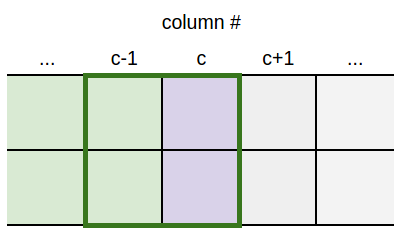
\includegraphics[width=0.35\textwidth]{scrabble/imgs/scrabble-per-column}
		\captionsetup{width=0.8\textwidth}
	\caption{Jika $ S $ dapat ditemukan pada petak-petak dalam kotak hijau, maka pengisian $ N-c $ kolom sisanya dapat diabaikan (daerah abu-abu).}
\end{figure*}

Perhatikan bahwa pada optimisasi ini, untuk mengisi petak-petak pada suatu kolom $ c $ dibutuhkan pula informasi mengenai karakter-karakter pada kolom sebelumnya (kolom $ c - 1 $) untuk dapat membantu menentukan dibentuk-tidaknya $ S $.

Solusi ini akan dioptimisasi lebih lanjut dengan \textit{dynamic programming} pada subbagian editorial berikutnya.

Batasan kedua versi: $1 \le N \le 50; 1 \le K \le 26$

\subsection*{Versi Mudah}
\addcontentsline{toc}{subsection}{Versi Mudah} % for pdf indexing
Batasan: $\mathbf{|S| = 2}$

Dari penjelasan pada subbagian sebelumnya, perhatikan bahwa suatu \textit{state}/keadaan pengisian petak-petak rubrik petakata dapat direpresentasikan dengan komponen-komponen berikut.

\begin{itemize}
\item $ c $, yang menyatakan posisi kolom yang sedang/akan diisi, dan
\item $ (k'_1, k'_2) $, yaitu karakter-karakter pengisi kolom ke-$ (c-1) $.
\end{itemize}

Dengan menerapkan \textit{dynamic programming} (memoisasi terhadap \textit{state} dan hasil) pada \textit{state} di atas dan menggunakan transisi yang serupa pada solusi pada subbagian Pra-Versi Mudah, maka kompleksitas solusi yang didapat adalah $ \bigO{NK^2 \cdot K^2} = \bigO{NK^4} $. Untuk lebih jelasnya, berikut relasi rekurensi dari \textit{dynamic programming} yang diterapkan:

$$
\dpf(c, k'_1, k'_2) = 
\begin{cases} 
	0, & c > N\\
	\displaystyle \sum_{\substack{a, b \in A_K\\\mathrm{canMakeS}(k'_1, k'_2, a, b)}} K^{2(N-c)} 
	+ \displaystyle \sum_{\substack{a, b \in A_K\\\lnot\mathrm{canMakeS}(k'_1, k'_2, a, b)}} \dpf(c + 1, a, b), & c \le N
\end{cases}
$$

dengan $ \mathrm{canMakeS}(p, q, r, s) $ bernilai $ \mtrue $ jika salah satu dari $ pr, ps, qr, qs, rs, $ atau $ sr $ membentuk $ S $.

Jawaban terdapat pada $ \dpf(1, -, -) $ dengan $ - $ adalah karakter yang tidak terdapat dalam $ A_K $. Karakter $ - $ dipilih dikarenakan pada \textit{state} pada kolom pertama, tidak terdapat karakter yang sebelumnya telah terpasang (tidak terdapat karakter pada kolom ke-$ 0 $).

\subsection*{Versi Sulit}
\addcontentsline{toc}{subsection}{Versi Sulit} % for pdf indexing

Batasan: $\mathbf{1 \le |S| \le 10}$

Solusi untuk versi mudah tidak dapat secara langsung diperumum/diterapkan untuk menyelesaikan versi sulit karena terdapat batasan bahwa untuk suatu masukan $ S $, dalam pengisian petak-petak pada kolom $ c $ dibutuhkan informasi mengenai karakter-karakter yang mengisi kolom-kolom $ c-|S|+1 $ hingga $ c-1 $, yang mengakibatkan kompleksitas solusi menjadi $ \bigO{NK^{2|S|} \cdot {K^2}} = \bigO{NK^{2(|S| + 1)}} $. Untuk versi ini, $ |S| $ dapat mencapai 10; penerapan solusi versi mudah secara langsung memiliki kompleksitas $ \bigO{NK^{22}} $ yang akan mendapatkan penilaian \textit{Time Limit Exceeded} pada versi sulit.

\subsubsection*{Algoritma KMP}
\addcontentsline{toc}{subsubsection}{Algoritma KMP} % for pdf indexing

Algoritma Knuth-Morris-Pratt (KMP) adalah salah satu algoritma pencarian \textit{string}. Silakan merujuk pada literatur terkait untuk mengetahui lebih lanjut mengenai algoritma tersebut.

Himpunan \textit{state} dalam suatu eksekusi algoritma KMP untuk mencari suatu string $ S $ dalam suatu teks $ T $ dapat direpresentasikan dalam suatu \textit{deterministic finite state machine} (DFSM). Sebagai contoh, DFSM dalam eksekusi algoritma KMP untuk mencari $ S =\texttt{tesate} $ adalah sebagai berikut.

\begin{center}
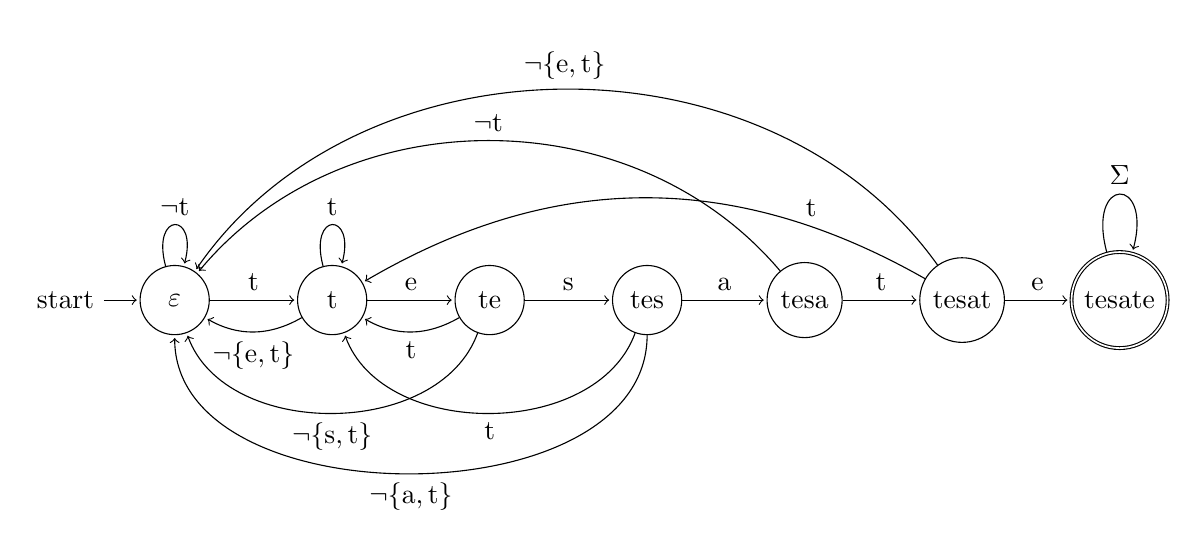
\begin{tikzpicture}[shorten >=1pt,node distance=2cm,on grid,auto] 
	\node[state,initial] (q_0)   {$ \varepsilon $}; 
	\node[state] (q_1) [right=of q_0] {t};
	\node[state] (q_2) [right=of q_1] {te};
	\node[state] (q_3) [right=of q_2] {tes};
	\node[state] (q_4) [right=of q_3] {tesa};
	\node[state] (q_5) [right=of q_4] {tesat};
	\node[state,accepting](q_6) [right=of q_5] {tesate};
	\path[->] 
	(q_0) edge  node {t} (q_1)
		  edge [loop above] node {$ \lnot $t} ()
	(q_1) edge  node  {e} (q_2)
		  edge [loop above] node {t} ()
		  edge [bend left] node {$ \lnot \{\mathrm{e, t}\} $} (q_0)
	(q_2) edge  node  {s} (q_3)
		  edge [bend left] node {t} (q_1)
		  edge [bend left=70] node {$ \lnot \{\mathrm{s, t}\} $} (q_0)
	(q_3) edge  node  {a} (q_4)
	      edge [bend left=70] node {t} (q_1)
	      edge [bend left=90] node {$ \lnot \{\mathrm{a, t}\} $} (q_0)
	(q_4) edge  node  {t} (q_5)
	      edge [bend right=50] node[above] {$ \lnot \mathrm{t} $} (q_0)
	(q_5) edge  node  {e} (q_6)
	      edge [bend right=30] node[above,pos=0.2] {t} (q_1)
   	      edge [bend right=55] node[above] {$ \lnot \{\mathrm{e, t}\} $} (q_0)
   	(q_6) edge [loop above] node {$ \Sigma $} ()
	;
\end{tikzpicture}
\end{center}

Perhatikan bahwa untuk suatu string $ S $, maka DFSM yang terbentuk akan memiliki tepat $ |S| + 1 $ \textit{state}. Untuk DFSM di atas, string $ S $ dikatakan ditemukan dalam teks $ T $ apabila \textit{state} pada akhir eksekusi algoritma KMP adalah pada \textit{state} akhir (\textit{state} dengan dua garis pinggir).

Sebagai kesepakatan, berikut beberapa notasi terkait DFSM.

\begin{itemize}
\item $ Q $, menyatakan himpunan \textit{state} dalam DFSM.
\item $ \Sigma $, menyatakan himpunan karakter/masukan dalam DFSM.
\item $ \delta : Q \times \Sigma \rightarrow Q $, menyatakan transisi dalam DFSM.
\item $ q_0 $, menyatakan \textit{state} awal/mulai.
\item $ A $, menyatakan himpunan \textit{state} akhir/selesai.
\end{itemize}

Dalam contoh DFSM untuk $ S = \texttt{tesate} $ di atas, maka

\begin{itemize}
\item
$ Q = \{q_\epsilon, q_t, q_{te}, q_{tes}, q_{tesa}, q_{tesat}, q_{tesate}\} $,
\item 
$ \Sigma = \{a, b, c, \mathellipsis\} $
\item
$ \delta = \{((q_\epsilon, \lnot t), q_\epsilon), ((q_\epsilon, t), q_t), ((q_t, t), q_t), ((q_t, e), q_{te}), \mathellipsis\} $
\item $ q_0 = q_\epsilon $
\item $ A = \{q_{tesate}\} $.
\end{itemize}

\subsubsection*{Solusi untuk Petak Berukuran $ 1 \times N $}
\addcontentsline{toc}{subsubsection}{Solusi untuk Petak Berukuran $ 1 \times N $} % for pdf indexing

Jika soal yang diberikan tetap sama namun petak yang diberikan berukuran $ 1 \times N $, maka salah satu solusi yang dapat menyelesaikan varian ini adalah dengan terlebih dahulu membangun DFSM untuk string $ S $ dan menggunakan \textit{dynamic programming} dengan komponen-komponen \textit{state}

\begin{itemize}
\item $ c $, yang menyatakan posisi kolom yang sedang/akan diisi, dan
\item $ q $, \textit{state} DFSM yang dicapai pada pengisian kolom ke-$ (c-1) $ setelah mengisi ke-$ (c - 1) $ kolom sebelumnya.
\end{itemize}

serta dengan relasi rekurensi

$$
\dpf(c, q) = 
\begin{cases}
	0, & c > N + 1\\
	0, & c = N + 1\land q \not\in A\\
	1, & c = N + 1\land q \in A\\
	\displaystyle \sum_{k \in A_K} \dpf(c + 1, \delta(q, k)), & c \le N.
\end{cases}
$$

Perhatikan bahwa \textit{base case} yang memiliki nilai kembalian $ 1 $ terjadi pada kasus dengan $ c = N + 1 \land q \in A $, yaitu saat seluruh petak telah terisi karakter dan terdapat string $ S $ pada petak-petak yang telah terisi.

Jawaban terdapat pada $ \dpf(1, q_0) $. Solusi ini memiliki kompleksitas $ \bigO{\textrm{pembangunan DFSM untuk }S} + \bigO{\textrm{eksekusi solusi dengan DP}} = \bigO{|S|} + \bigO{NK^2} = \bigO{|S| + NK^2} $.

\subsubsection*{Solusi untuk Petak Berukuran $ 2 \times N $ (Soal Versi Sulit)}
\addcontentsline{toc}{subsubsection}{Solusi untuk Petak Berukuran $ 1 \times N $} % for pdf indexing

Solusi untuk varian petak berukuran $ 1 \times N $ di atas dapat dikembangkan menjadi solusi untuk soal versi sulit dengan melakukan modifikasi terhadap komponen-komponen \textit{state} dari \textit{dynamic programming} yaitu

\begin{itemize}
\item $ c $, menyatakan posisi kolom yang sedang/akan diisi, dan
\item $ V $, menyatakan himpunan \textit{state} DFSM yang mungkin dicapai jika telah melakukan pengisian pada ke-$ (c - 1) $ kolom sebelumnya dan berakhir pada posisi baris manapun pada kolom ke-$ (c - 1) $
\end{itemize}

dan dengan relasi rekurensi sebagai berikut.

$$
\dpf(c, V) = 
\begin{cases}
	0, & c > N + 1\\
	0, & c = N + 1\land A \cap V = \varnothing \\
	1, & c = N + 1\land A \cap V \neq \varnothing \\
	\displaystyle \sum_{a,b \in A_K} \dpf \left(c + 1, \bigcup\limits_{q \in V} \left(\left\{\delta\left(q, a\right), \delta\left(q, b\right), \delta\left(\delta\left(q, a\right), b\right), \delta\left(\delta\left(q, b\right), a\right) \right\} \right) \right), & c \le N.
\end{cases}
$$

Karena banyak maksimal elemen berbeda dari $ V $ adalah $ |S| + 1 $, maka secara implementasi $ V $ dapat dinyatakan dalam \textit{bitmask}.

Dalam pengerjaannya, implementasi naif untuk menghitung $ \bigcup_{q \in V}\delta(q, a) $ dalam transisi pada kasus keempat dalam relasi rekurensi di atas memiliki kompleksitas sebesar $ \bigO{|S|} $. Hal tersebut dapat dioptimisasi dengan melakukan prekomputasi terhadap pemetaan $ \delta^\ast : \powerset{Q} \times \Sigma \rightarrow \powerset{Q} $ sehingga untuk suatu himpunan \textit{state} $ V $ dan karakter $ a $, penghitungan $ V' = \bigcup_{q \in V} \delta(q, a) $ dapat dilakukan dalam $ O(1) $, yaitu $ V' = \delta^\ast(V, a) $.

Bentuk relasi rekurensi yang telah dioptimisasi:

$$
\dpf(c, V) = 
\begin{cases}
	0, & c > N + 1\\
	0, & c = N + 1\land A \cap V = \varnothing \\
	1, & c = N + 1\land A \cap V \neq \varnothing \\
	\displaystyle \sum_{a,b \in A_K} \dpf \left(c + 1, \delta^\ast\left(V, a\right) \cup \delta^\ast\left(V, b\right) \cup \delta^\ast\left(\left(V, a\right), b\right) \cup \delta^\ast\left(\left(V, b\right), a\right) \right), & c < N + 1.
\end{cases}
$$

Jawaban terdapat pada $ \dpf\left(1, \left\{q_\epsilon\right\} \right) $ Solusi ini memiliki kompleksitas sebesar $ \bigO{\textrm{pembangunan DFSM untuk }S} + \bigO{\textrm{\textit{state} DP}} \cdot \bigO{\textrm{transisi DP}} = \bigO{|S|} + \bigO{N2^{|S| + 1}} \cdot \bigO{K^2} = \bigO{|S| + NK^22^{|S| + 1}} $.

\end{document}
